%% Files that are needed for LaTeX processing (style + inputs) are available
%% relative to the download place in the directory ../inputs, the images in
%% ../img

\documentclass[compress]{beamer}

\usepackage[utf8]{inputenc}
\mode<presentation>{
   \usetheme{Boadilla}
   \hypersetup{pdfpagemode=FullScreen}
}
\setbeamertemplate{navigation symbols}{}

\usepackage{debian-links}

\title{Debian Teams Activity Metrics}

\author{Andreas Tille and Sukhbir Singh}

%\institute{\Debian}
\institute{\link{http://www.debconf.org/debconf11/}{Debian Conference 11}}

\date{Banja Luka, Bosnia and Herzegovina, July 29, 2011}

\begin{document}

\begin{frame}
  \titlepage
\end{frame}

\section{Short historical introduction}

\begin{frame}
  \frametitle{Motivation}

  \begin{itemize}
     \item Who is inside the team?
     \item Who left the team?
     \item Does a team have enough members?
     \item Is the team growing or shrinking?
  \end{itemize}
\end{frame}

\begin{frame}
  \frametitle{Quite simple start: Mailing list activity}
      \begin{center}
        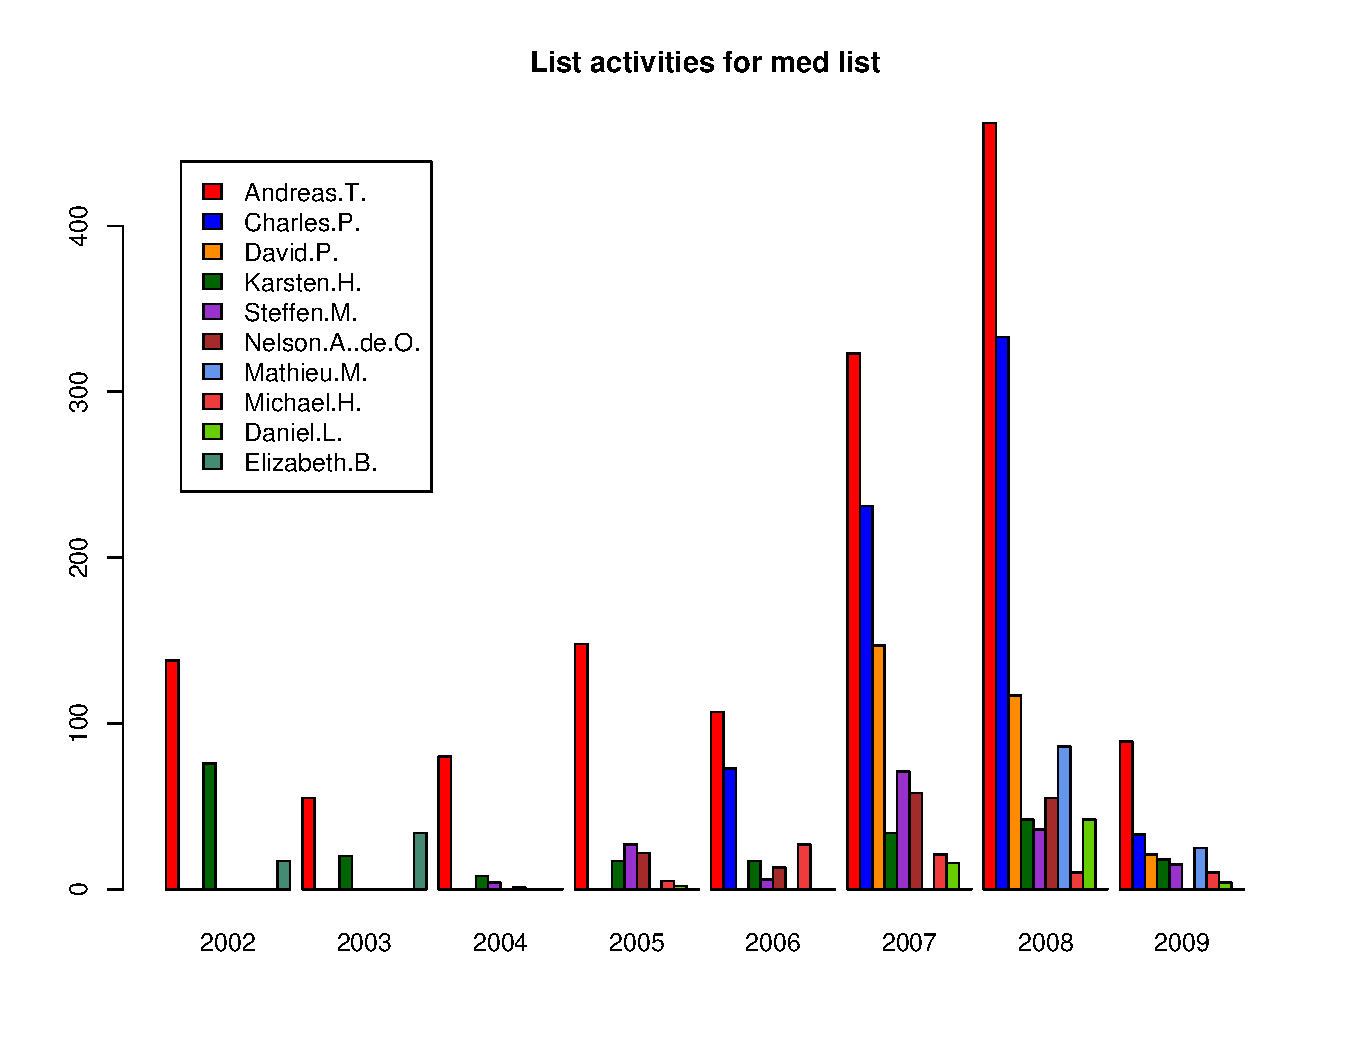
\includegraphics[width=0.9\textwidth]{authorstat_med}
      \end{center}

\end{frame}

\begin{frame}
  \frametitle{Measure of Communication Activity}

  \begin{itemize}
     \item Every project has a mailing list
     \item We measure who are the most active contributors
     \item Quantity is not the only metric because quality matters 
     \item We handle spam by filtering it
  \end{itemize}

\end{frame}

\begin{frame}
 \frametitle{Metrics for Measuring Performance}

 \begin{itemize}
    \item Frequency of posting 
    % Indicate that this is a quantitative metric. 
    \item The raw length of the message body 
    % These are all qualititative metrics and the length of the message body is common to all these.  
    % The length of the message body excluding: 
    \item blank lines 
    \item blank lines and quotes
    % Indicate that this is the most solid metric of all. 
    \item blank lines, quotes and signatures
 \end{itemize}
\end{frame}


% Debian Edu
\begin{frame}
  \frametitle{Top 10 \link{http://lists.debian.org/debian-edu}{debian-edu@lists.debian.org}}
   \vspace{-5mm}

      \begin{center}
        \resizebox{125mm}{90mm}{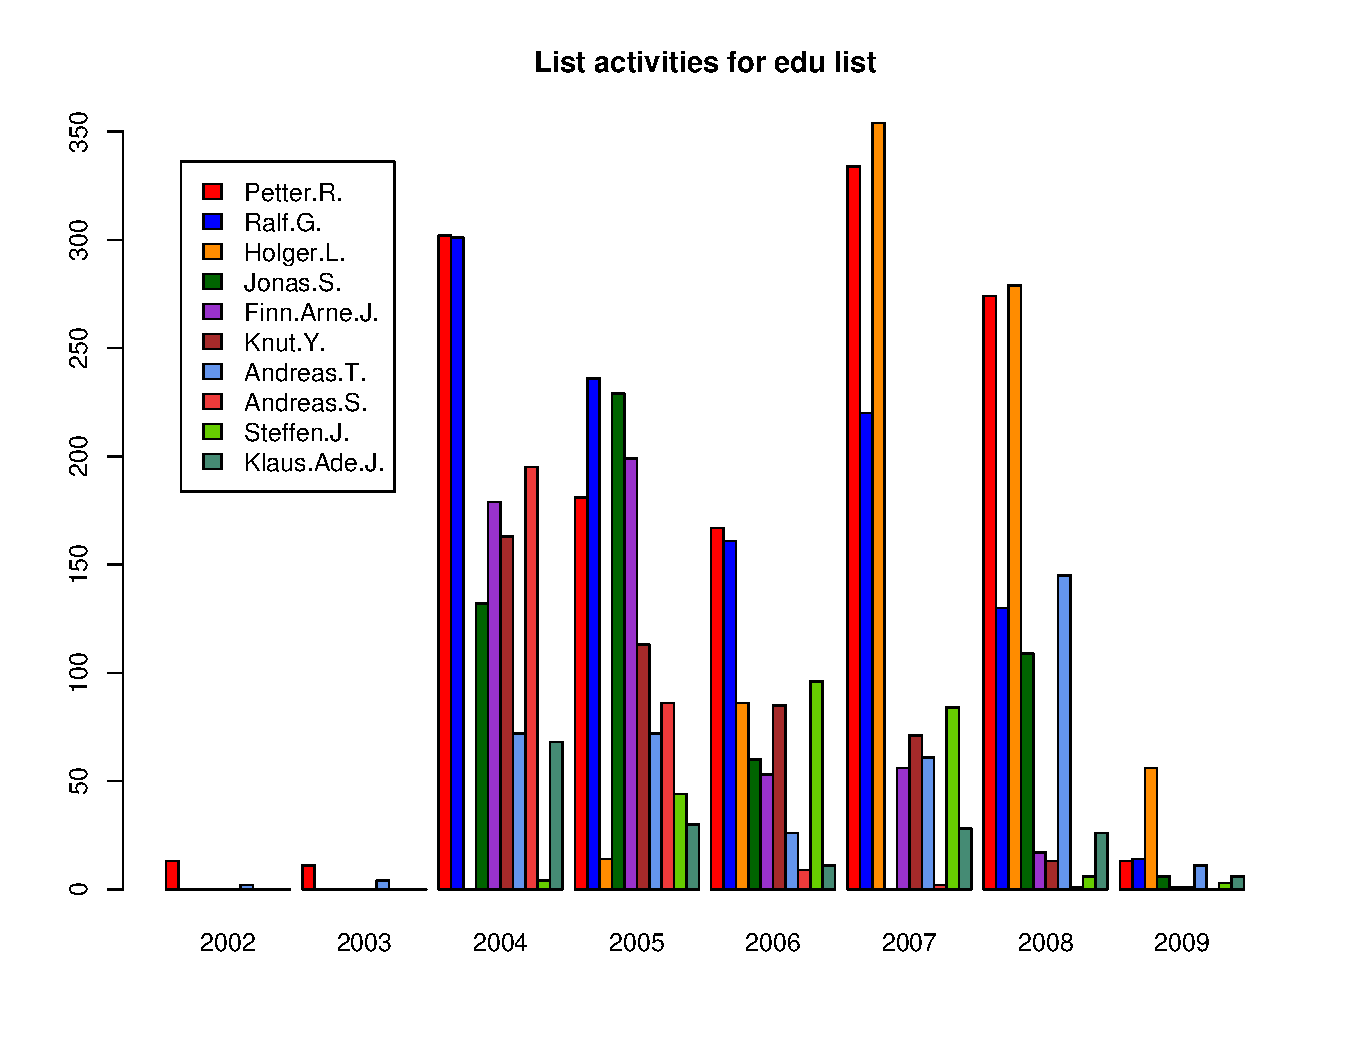
\includegraphics{authorstat_edu}}
      \end{center}

\end{frame}

% Debian Jr
\begin{frame}
  \frametitle{Top 10 \link{http://lists.debian.org/debian-jr}{debian-jr@lists.debian.org}}
   \vspace{-5mm}
        
      \begin{center}
        \resizebox{125mm}{90mm}{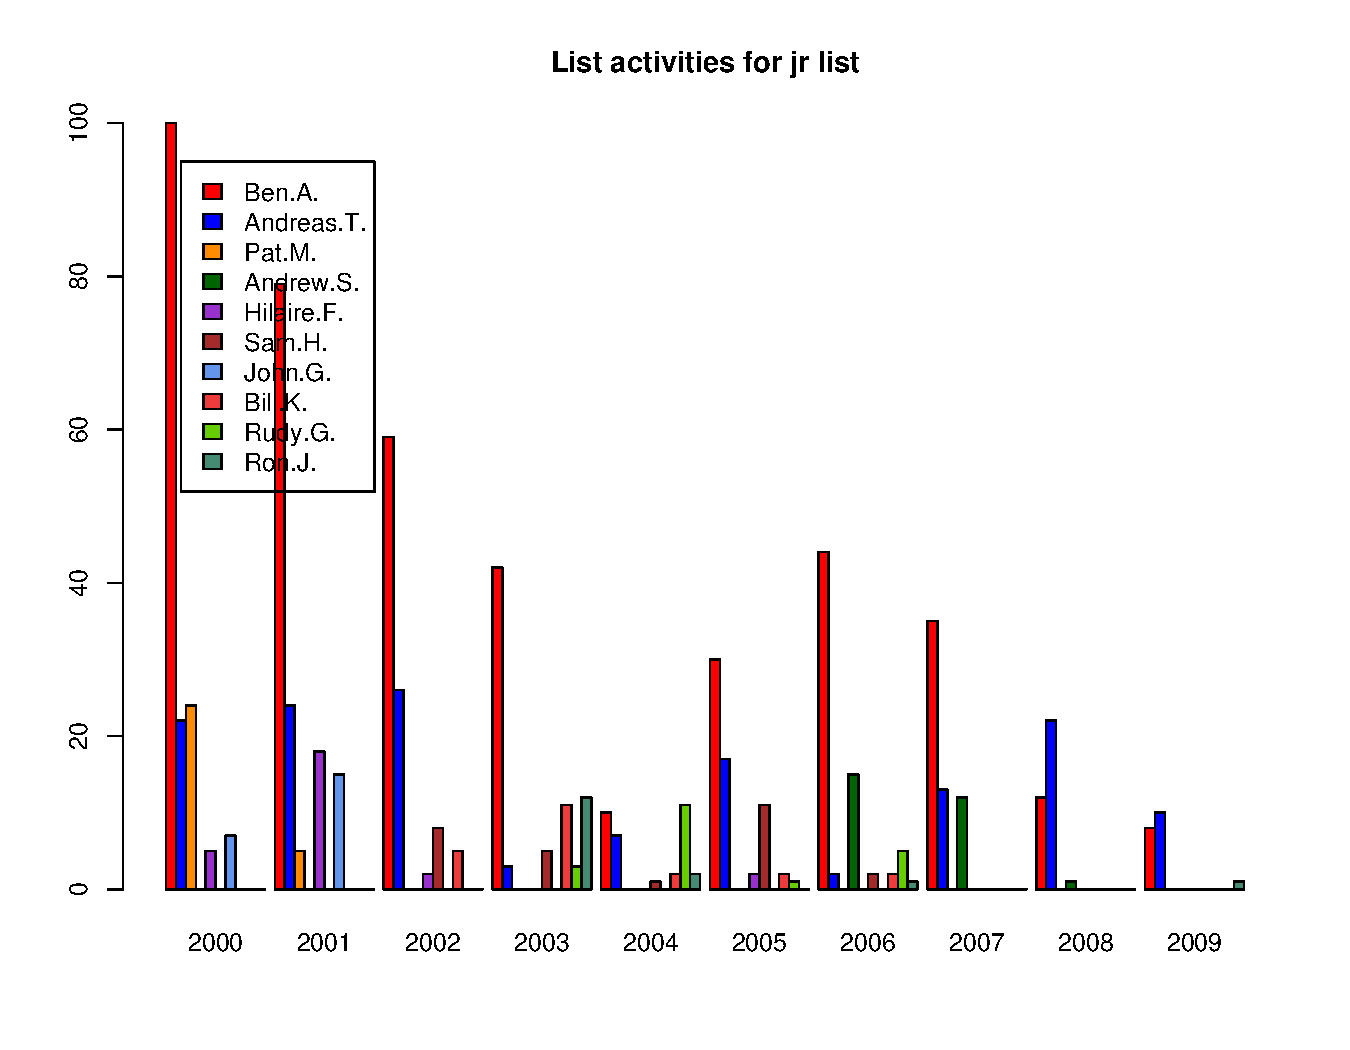
\includegraphics{authorstat_jr}}
      \end{center}
      
\end{frame}

% Debian Enterprise
\begin{frame}
  \frametitle{Top 10 \link{http://lists.debian.org/debian-enterprise}{debian-enterprise@lists.debian.org}}
   \vspace{-5mm}

      \begin{center}
        \resizebox{125mm}{90mm}{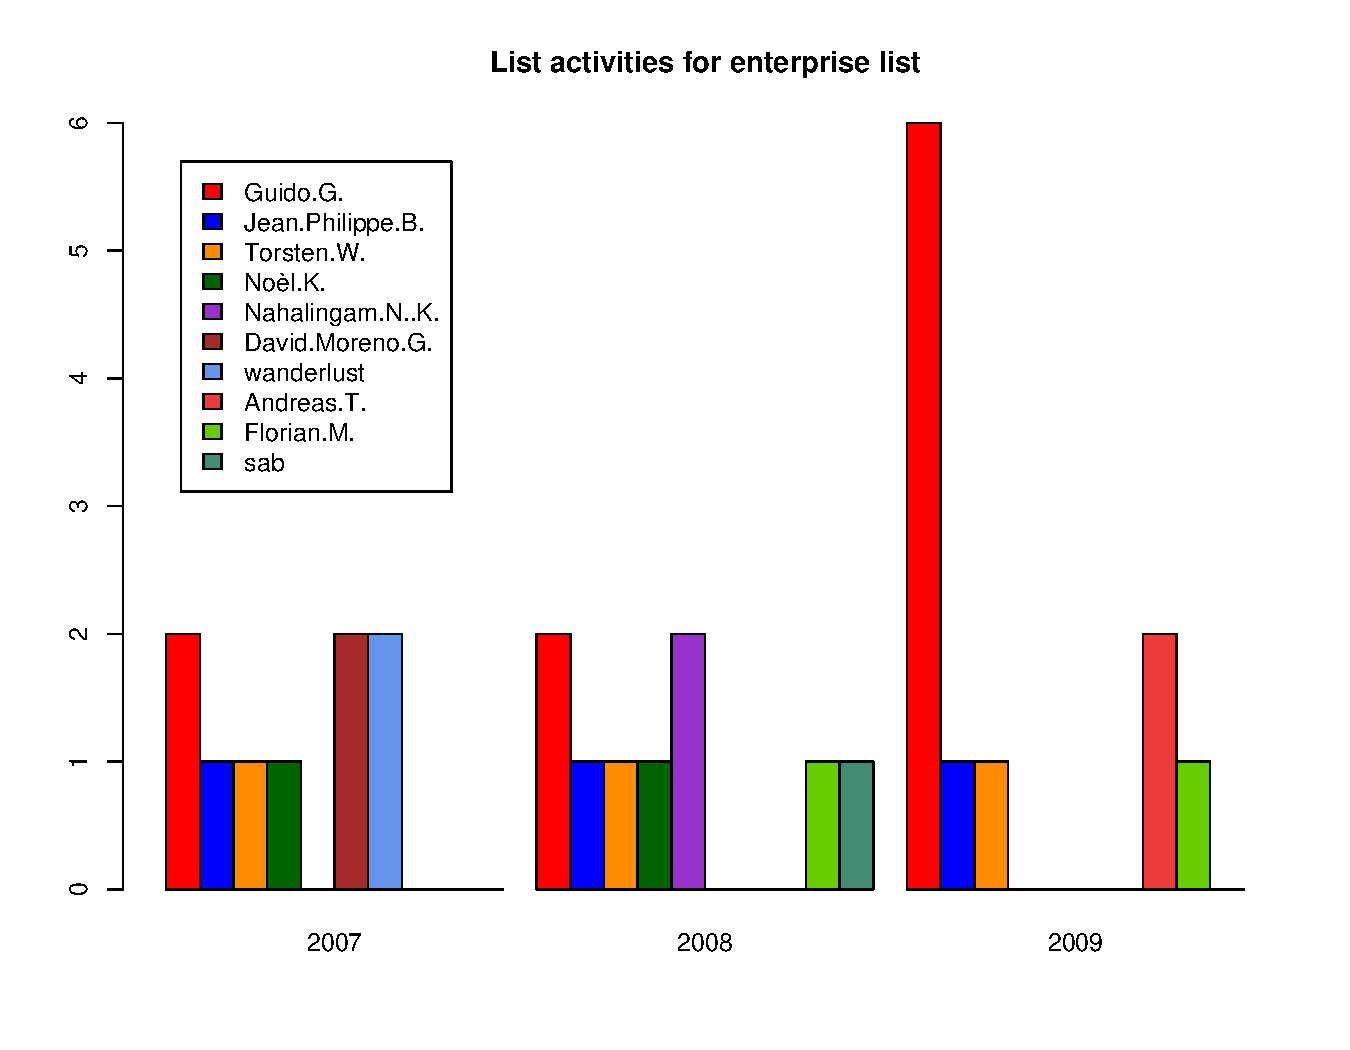
\includegraphics{authorstat_enterprise}}
      \end{center}
      
\end{frame}

%\input med-end-en.tex

\end{document}

